
\chapter{Method}

\section{Model Intuition}
\label{mod:intuition}
The model that is developed in this thesis consists of two parts. As a first step, Matrix Factorization (\textit{MF}) is applied to make a first prediction on the missing drug-target pairs. \textit{MF} predicts the missing values based only on the observations in the training dataset and does not take additional features of the drugs and targets into account. This is where the second part of the model, Continuous Conditional Random Fields (\textit{CCRF}) comes into play. The \textit{CCRF} gets the similarity matrices of the drugs and targets as input, together with the training dataset, the predictions that were made by \textit{MF} on the missing values and the predictions that were made by \textit{MF} on the training data ($MF$ is applied twice, to make predictions on missing values and the training data itself as described below). The intuition behind the \textit{CCRF} is to re-predict the missing values based on three parameters $\alpha$, $\beta_1$, $\beta_2$ which represent respectively:
\begin{itemize}
\item $\alpha$: the \textit{trustworthiness} of the \textit{MF} prediction. 
\item $\beta_1$: how much can be interpolated between drug-drug pairs with high similarity scores in the drug similarity matrix.
\item $\beta_2$: how much can be interpolated between target-target pairs with high similarity scores in the target similarity matrix.
\end{itemize}
The trustworthiness of the \textit{MF} prediction is learned from the training data and the predictions that were made by \textit{MF} on these data points. The dependance of drug-drug and target-target pairs with high similarity is captured by learning how similar the binding values of these pairs are in the training data. The idea of the combined \textit{MF+CCRF} model is that the \textit{CCRF} can improve the initial \textit{MF} prediction of a drug-target pair by interpolating from given observations of a similar drug on the same target or by interpolating from a given observation of a similar target on the same drug. When it is not possible to interpolate from a given observation to make a prediction for a drug-target pair, the combined model will just fall back onto the initial $MF$ prediction.

The two parts of the model, \textit{MF} and \textit{CCRF} are described first separately and then in combination in the following sections. Matrix Factorization is described in section \ref{sec:MF}. \textit{CCRF} is described in more detail in section \ref{sec:CCRF}. Both, \textit{MF} and \textit{CCRF} are explained by first giving a short overview, then explaining the parameter learning step and finally describing how missing values can be predicted (the inference step).
The combination of the two models (\textit{MF+CCRF}) is described in section \ref{sec:MFCCRF}. This thesis focuses mainly on the \textit{CCRF} part of the \textit{MF+CCRF} model. Before going into the model details, section \ref{sec:Notation} gives an overview of the used notation.

\section{Notation}
\label{sec:Notation}
Let $D$ and $T$ denote sets of drugs and targets respectively. Let $R \in \mathbb{R} ^{|D| \times |T|}$ denote a drug-target interaction matrix, where the rows represent the drugs in $D$ and the columns represent the targets in $T$. $R$ contains missing values for drug-target pairs for which the interaction strength is unknown and real values representing the interaction strength for drug-target pairs whose binding affinity was measured in wetlab experiments. The known values in $R$ serve as training data for the developed model and the missing values are those that we wish to predict. Further, let $S_D \in \mathbb{R}^{|D| \times |D|}$ and $S_T \in \mathbb{R}^{|T| \times |T|}$ denote matrices containing similarity scores for the drugs $D$ and targets $T$ respectively. The interaction data and similarity scores can be of different kind as described in section \ref{sec:datasets}.  In the \textit{drug-target interaction prediction} task, the number of missing values in $R$ usually outweights the number of known interactions and $R$ is only sparsely populated.

\section{Matrix Factorization}
\label{sec:MF}
The Matrix Factorization technique has been demonstrated to be effective specially for personalized recommendation tasks \cite{Koren:2009:MFT:1608565.1608614} and it has been previously applied for drug-target interaction prediction \cite{liu2016neighborhood}, \cite{ezzat2016drug}, \cite{gonen2013kernelized}. Here, the \textit{MF} technique is utilized in its simplest form, without incorporating the similarity matrices directly as it is done in \cite{liu2016neighborhood} and \cite{gonen2013kernelized}. \textit{MF} is a process in which the sparsely filled training matrix $R$ is approximated by the product of two factor matrices $P \in \mathbb{R}^{k\times |D|}$ and $Q \in \mathbb{R}^{k\times |T|}$ as described in the following two sections.

\subsection{Parameter Learning}

The factor matrices $P$ and $Q$ are learned by minimizing the regularized squared error on the set of known affinities $\kappa$:
\begin{equation}
\min\limits_{Q,P}{\sum\limits_{(d_i,t_j)\in \kappa} (a_{i,j}-q_i^Tp_j)^2} + \lambda (||p||^2 + ||q||^2)
\end{equation}
The term $(a_{i,j}-q_i^Tp_j)^2$ represents the fit of the learned parameters to the previously observed binding affinites. The term $\lambda (||p||^2 + ||q||^2)$ penalizes the magnitudes of the learned parameters to prevent overfitting and the constant $\lambda$ controls the extend of overfitting.
The above optimization problem can be solved by stochastic gradient descent as described in \cite{Koren:2009:MFT:1608565.1608614}:
The algorithm loops through all pairs $(d_i, t_j)$ in $R$ for which the binding affinity is known, computes the current prediction for $(d_i, t_j)$ and computes the associated prediction error as:
\begin{equation}
e_{i,j} = r_{i,j} - p_i^Tq_j
\end{equation}
where $p_i$ denotes the $i$th column of $P$ and $q_j$ denotes the $j$th column of $Q$. The columns of $P$ and $Q$ are then modified in the opposite direction of the gradient:
\begin{equation}
p_i:= q_i + \gamma (e_{i,j} p_j - \lambda q_i)
\end{equation}
\begin{equation}
q_j:=p_i + \gamma (e_{i,j} p_i - \lambda q_j)
\end{equation}
where $\gamma$ is a constant specifying the magnitude of the update.

\subsection{Inference}

With learned matrices $P$ and $Q$, a missing affinity of drug-target pair $(d_i, t_j)$ in $R$ can be predicted by the inner product of the $i$th column of $P$ and the $j$th column of $Q$. A matrix $R'$ with predictions for all drug-target pairs can be computed as:
\begin{equation}
R' = P^TQ
\end{equation}

\section{Continuous Conditional Random Fields}
\label{sec:CCRF}

Conditional Random Fields were originally developed for the task of segmenting and labeling sequence data \cite{lafferty2001conditional}. In contrast to predicting continuous values as for drug-target binding affinities, the original formulation predicts a label vector $Y$, where all components of $Y_i$ are assumed to range over a finite label alphabet $\mathcal{Y}$. For the task of classifying whether or not a drug-target pair is interacting, CRFs were applied previously \cite{yang2014drug}.

%(non-continuous) Conditional Random Fields were applied successfully for tasks, such as ...

To the best of my knowledge, the continuous variant of Conditional Random fields were first introduced by \cite{qin2009global} for ranking tasks in document retrieval systems. An other application of \textit{CCRFs} for recommender systems can be found in \cite{xin2009social}. The problem formulation in \cite{xin2009social} is very similar to the problem of drug-target interaction prediction. However the formulation in \cite{xin2009social} requires taking a Gibbs-sample of the distribution defined through the \textit{CCRF} in each update step during parameter learning. Although with the drawback of reducing the feasible size of the graphical model, \cite{baltruvsaitis2013dimensional} presents a closed form solution for the parameter learning and inference step. This closed formulation of the \textit{CCRF} is applied for the model that is used in this thesis. The following sections formally describe the \textit{CCRF} and explain the parameter learning and the inference step.


%In the non-continuous formulation, label sequences $Y$ are modeled as a conditional distribution $P(Y|X)$.

%describe difference to HMMs [In contrast to the generative Hidden Markov Models, defining a joint probability over observation and label sequences, which require to enumerate all possible observation sequences, a conditional model specifies the probabilities of possible label sequences \textbf{given} an observation sequence. Therefore a conditional model does not expend modeling effort on the observations.]

%Conditional Random Fields model a sequence of labels $Y$, given an observation vector $X$ as a conditional probability $P(Y|X)$. In non-continuous CRFs, the components $Y_i$ of $Y$ are assumed to range over a finite label alphabet $\mathcal{Y}$.


\subsection{Formal Definition}
Here I will use the same notation as it is presented in \cite{baltruvsaitis2013dimensional}. A \textit{CCRF} is an undirected graphical model which models a set of output variables $Y=\{y_1,\dots,y_n\}$, $y_i \in \mathbb{R}$ that we wish to predict as $P(Y|X)$ where  $X=\{x_1,\dots,x_n\}$, $x_i \in \mathbb{R}^m$ is a set of observed input variables. The \textit{CCRF} defines a conditional probability distribution with the density function:
\begin{equation}\label{eq:CCRF_main}
P(Y|X)=\frac{\text{exp}(\Psi)}{\int_{-\infty}^{\infty} \text{exp}(\Psi) dy}
\end{equation}
\begin{center}
$\Psi=\sum_i \sum\limits_{k=1}^{K_1} \alpha_k f_k(y_i, X) + \sum_{i,j} \sum \limits_{k=1}^{K_2} \beta_k g_k (y_i, y_j,X)$
\end{center}
The term $\int_{-\infty}^{\infty}\text{exp}(\Psi) dy$ is a normalization term which makes the probability distribution valid. The $f_k$ terms will be called vertex features and the $g_k$ terms edge features. The feature functions are defined as:
\begin{center}
$f_k(y_i,X) = -(y_i - X_{i,k})^2$\\
$g_k(y_i,y_j,X) = -\frac{1}{2}S_{i,j}^k(y_i - y_j)^2$
\end{center}
Intuitively, the weights $\alpha_k$ on the feature functions $f_k$ represent the reliability of observation $X_{i,k}$ in regard to the true label $y_i$. Here, the observations $X_{i,k}$ can for example represent the initial predictions of a set of $K_1$ regressors. In the \textit{CCRF} that is used for the experiments in this thesis there is always only one regressor (and thus $K_1=1$) which is the Matrix Factorization part of the model and $X_{i,1}$ represents the initial prediction coming from Matrix Factorization.  Edge features $g_k$ represent the dependency between labels $y_i$ and $y_j$ with similarity $S_{i,j}^k, k \in 1,\dots, K_2$. With given drug-drug similarity matrix $S_D$ and target-target similarity matrix $S_T$, $S_{i,j}^1$ and $S_{i,j}^2$ can for example be defined as:
\begin{equation}
\label{simi_1}
S_{i,j}^1 =
\begin{cases}
1, & S_D(i,j) > thresh_d \\
0, & S_D(i,j) < thresh_d
\end{cases} 
\end{equation}
\begin{equation}
\label{simi_2}
S_{i,j}^2 =
\begin{cases}
1, & S_T(i,j) > thresh_t \\
0, & S_T(i,j) < thresh_t
\end{cases} 
\end{equation}
where $thresh_d$ and $thresh_t$ are user defined thresholds. Intuitively, the weights $\beta_1$ and $\beta_2$ on $S_{i,j}^1$ and  $S_{i,j}^2$ respectively, now represent the importance of assigning similar prediction values to drug pairs with similarity larger than $thresh_d$ and of assigning similar prediction values to target pairs with similarity larger than $thresh_t$. Note, that the dimensions of $S^k$ and the similarity matrices $S_D$ and $S_T$ are usually different. The matrices $S^k$ contain as many rows and columns as there are nodes in the graphical structure of the \textit{CCRF}. Here $S_D(i,j)/S_T(i,j)$ refers to the similarity of the drugs/targets that correspond to the nodes $i$ and $j$ in the graphical structure.

As explained in the following sections, the conditional probability distribution that is defined through the \textit{CCRF} can be transformed into a multivariate Gaussian distribution in closed form, which is a useful property for both learning the weights on the feature functions as well as making predictions for missing values.
\subsection{Parameter Learning}

This section describes the parameter learning procedure of the \textit{CCRF} for quadratic vertex and edge functions as described above. Assume, we are given training values $Y=\{y_1,\dots,y_n\}$. Additionally, for each $y_i$ we have given the prediction $X_{i,k}$ that regressor $k$ would have predicted. As explained above, for the model in this thesis we have $K_1=1$ and thus we have only one prediction $X_{i,1}$ for each training data point, which is the Matrix Factorization prediction. Further we have $K_2$ similarity matrices given, which in the scope of this thesis can for example be the matrices $S_{i,j}^1$ and $S_{i,j}^2$ as defined in equation \ref{simi_1} and equation \ref{simi_2} respectively. In the learning step, we want to find the $\alpha$ and $\beta_k$ weights, that optimize the conditional log-likelihood of the \textit{CCRF} on the training data:

\begin{equation}  
\label{eq:log_likelihood}
L(\alpha,\beta)=\text{log}P(Y|X)
\end{equation}
\begin{equation}  
(\alpha_{opt}, \beta_{opt}) = \argmax_{\alpha, \beta}(L(\alpha,\beta))
\end{equation}
Because this problem is convex \cite{qin2009global}, standard techniques such as stochastic gradient descent can be utilized to determine the optimal parameters $\alpha$ and $\beta_k$. For the computation of the derivatives of $\text{log}P(Y|X)$ it helps to convert equation \ref{eq:CCRF_main} into the form of a multivariate Gaussian distribution. The conversion into the Gaussian formulation and the computation of the derivatives are described in detail in the following two sections. The log-likelihood is optimized with respect to log$\alpha$ and log$\beta_k$ in order to guarantee that $\alpha>0$ and $\beta_k>0$, which in turn guarantees that the normalization function is integrable. Using the partial derivatives, the \textit{CCRF} learning algorithm is as follows (here it is assumed that we are learning one parameter $\alpha$ and two $\beta$ parameters ($\beta_1, \beta_2$). The two $\beta$ parameters describe the weight on the drug-similarity and the target-similarity matrix respectively) :

\begin{center}
\begin{algorithm}
\renewcommand\thealgorithm{}
\caption{CCRF learning algorithm}
\begin{algorithmic}
\Require: $\{X_{train}, Y_{train}, S_D = S^1, S_T = S^2\}$
\State Params: number of iterations T, learning rate $\eta$
\State Initialise Parameters $\alpha$ and $\beta$
\For{$r=1$ to T } 
\State Compute current gradients with respect to log$\alpha$, log$\beta_1$, log$\beta_2$
\State log$\alpha$ = log$ \alpha+\eta\frac{\delta \text{log}(P(Y|X))}{\delta \text{log} \alpha}$
\State log$\beta_1$ = log$ \beta_1 + \eta\frac{\delta \text{log}(P(Y|X))}{\delta \text{log} \beta_1}$
\State log$\beta_2$ = log$ \beta_2 + \eta\frac{\delta \text{log}(P(Y|X))}{\delta \text{log} \beta_2}$
\State Update $\alpha$, $\beta_1$, $\beta_2$
\EndFor
\State Return $\alpha$, $\beta_1$, $\beta_2$
\end{algorithmic}
\end{algorithm}
\end{center}

\subsubsection{Gaussian Formulation of the CCRF}
This subsection describes the conversion of the probability distribution defined through equation \ref{eq:CCRF_main} into the formulation of a Gaussian distribution, as derived in \cite{baltruvsaitis2013dimensional}:

First, the feature functions are plugged into the energy function $\Psi$:

\begin{equation}
\label{learning:Psi}
\begin{split}
& \Psi = \sum\limits_{k=1}^{K1} \alpha_k f_k(y_i, X) + \sum_{i,j} \sum \limits_{k=1}^{K2} \beta_k g_k (y_i, y_j,X) \\
& = -\sum\limits_{k=1}^{K1} \alpha_k (y_i - X_{i,k})^2 - \frac{1}{2} \sum_{i,j} \sum \limits_{k=1}^{K2} \beta_k S_{i,j}^k(y_i-y_j)^2
\end{split}
\end{equation}

For the next step, we first define a diagonal matrix $A$ and a symmetric matrix $B$:
\begin{equation}
A_{i,j}=
\begin{cases}
\sum_{k=1}^{K_1} \alpha_k, & i=j\\
0, & i \neq j
\end{cases}
\end{equation}
\begin{equation}
B_{i,j} = 
\begin{cases}
(\sum_{k=1}^{K_2}\beta_k \sum_{r=1}^{n} S_{i,r}^k) - (\sum_{k=1}^{K_2} \beta_k S_{i,j}^{k}), & i=j \\
-\sum_{k=1}^{K_2} \beta_k S_{i,j}^k, & i \neq j
\end{cases}
\end{equation}
as well as 
\begin{equation}
\Sigma^{-1} = 2(A+B)
\end{equation}
and a vector $b$:
\begin{equation}
b_i = 2 \sum \limits_{k=1}^{K_1} \alpha_k X_{i,k}
\end{equation}
\begin{equation}
b = 2X\alpha
\end{equation}
The factor $\Psi$ in equation \ref{learning:Psi} can then be expressed in terms of $A, B$ and $b$:
First, terms of $\Psi$ containing $\alpha$ parameters are collected:

\begin{equation}
\begin{split}
& -\sum_i \sum \limits_{k=1}^{K_1} \alpha_k(y_i-X_{i,k})^2 \\
& = -\sum_i \sum \limits_{k=1}^{K_1} \alpha_k(y_i^2-2y_iX_{i,k}+X_{i,k}^2) \\
& = -\sum_i \sum \limits_{k=1}^{K_1} \alpha_k y_i^2 + \sum_i \sum\limits_{k=1}^{K_1} \alpha_k 2y_i X_{i,k} - \sum_i \sum\limits_{k=1}^{K_1} \alpha_k X_{i,k}^2\\
& = -y^TAy + y^Tb - \sum_i \sum\limits_{k=1}^{K_1} \alpha_k X_{i,k}^2
\end{split}
\end{equation}
Then, terms of $\Psi$ containing $\beta$ parameters are collected:
\begin{equation}
\begin{split}
& -\frac{1}{2}\sum_{i,j}\sum\limits_{k=1}^{K_2}\beta_k S_{i,j}^k(y_i-y_j)^2\\
& = -\frac{1}{2}\sum_{i,j}\sum\limits_{K=1}^{K_2}\beta_k S_{i,j}^k(y_i^2-2y_iy_j+y_j^2)\\
& = -\frac{1}{2}\sum_{i,j}\sum\limits_{K=1}^{K_2}\beta_k S_{i,j}(y_i^2+y_j^2) + \sum_{i,j} \sum\limits_{k=1}^{K_2}\beta_k S_{i,j}^ky_iy_j\\
& =  -\sum\limits_{k=1}^{K_2}\beta_k\sum_{i,j}S_{i,j}^ky_i^2 + \sum\limits_{k=1}^{K_2}\beta_kS_{i,j}^k\sum_{i,j}y_iy_j\\
& = -y^TBy
\end{split}
\end{equation}
Combining these we can write $\Psi$ as:
\begin{equation}
\Psi=-y^TAy + y^Tb - y^TBy - d = - \frac{1}{2}(y^T\Sigma^{-1}y)+y\Sigma^{-1}\mu - d
\end{equation}
where $d=\sum_i\sum\limits_{k=1}^{K_1}\alpha_kX_{i,k}^2$ and $\mu = \Sigma b$.

The $-d$ term can be cancelled out in the probability distribution:

\begin{equation}
\begin{split}
P(y|X)=& \frac{\text{exp}(\Psi)}{\int_{-\infty}^{\infty}\text{exp}(\Psi) dy}\\
& \frac{\text{exp}(- \frac{1}{2}(y^T\Sigma^{-1}y)+y\Sigma^{-1}\mu)\text{exp}(-d)}{\int_{-\infty}^{\infty}\text{exp}(- \frac{1}{2}(y^T\Sigma^{-1}y)+y\Sigma^{-1}\mu)\text{exp}(-d) dy} \\
& \frac{\text{exp}(- \frac{1}{2}(y^T\Sigma^{-1}y)+y\Sigma^{-1}\mu)}{\int_{-\infty}^{\infty}\text{exp}(- \frac{1}{2}(y^T\Sigma^{-1}y)+y\Sigma^{-1}\mu) dy} 
\end{split}
\end{equation}

The definite integral of $\text{exp}(- \frac{1}{2}(y^T\Sigma^{-1}y)+y\Sigma^{-1}\mu)$ with respect to $y$ can be found by using the formula for an integral with square and linear terms:
\begin{equation}
\text{exp}(- \frac{1}{2}(y^T\Sigma^{-1}y)+y\Sigma^{-1}\mu) = \frac{(2\pi)^{\frac{n}{2}}}{|\Sigma^{-1}|^{\frac{1}{2}}}\text{exp}(\frac{1}{2}\mu \Sigma^{-1} \mu)
\end{equation}

Finally, we obtain the Gaussian formulation of the probability distribution:

\begin{equation}
\begin{split}
P(y|X) = & \frac{\text{exp}(- \frac{1}{2}(y^T\Sigma^{-1}y)+y\Sigma^{-1}\mu)}{\frac{(2\pi)^{\frac{n}{2}}}{|\Sigma^{-1}|^{\frac{1}{2}}}\text{exp}(\frac{1}{2}\mu \Sigma^{-1} \mu)}\\
& \frac{\text{exp}( - \frac{1}{2} y^T \Sigma^{-1} y + y\Sigma^{-1}\mu )\text{exp} (-\frac{1}{2}\mu\Sigma^{-1}\mu) }{ (2\pi)^{\frac{n}{2}} |\Sigma|^{\frac{1}{2}} } \\
& \frac{\text{exp}(-\frac{1}{2} y^T \Sigma^{-1} y + y \Sigma^{-1} \mu - \frac{1}{2} \mu \Sigma^{-1} \mu)   }{  (2\pi)^{\frac{n}{2}} |\Sigma|^{\frac{1}{2}} } \\
& \frac{1}{   (2\pi)^{\frac{n}{2}} |\Sigma|^{\frac{1}{2}} }\text{exp}(-\frac{1}{2} (y-\mu)^T \Sigma^{-1} (y-\mu))
\end{split}
\end{equation}

\subsubsection{Partial Derivatives of the CCRF log-likelihood}

This section describes the calculation of the partial derivatives of the \textit{CCRF} log-likelihood with respect to the parameters $\alpha$ and $\beta$ as it is described in \cite{baltruvsaitis2013dimensional}.
The log-likelihood expressed as the Gaussian distribution as derived above is:

\begin{equation}
\begin{split}
\text{log}(P(y|X)) = & -\frac{1}{2}(y-\mu)^T \Sigma^{-1} (y-\mu) - \text{log}((2\pi)^{\frac{n}{2}}|\Sigma | ^{\frac{1}{2}}) \\
& = -\frac{1}{2}(y-\mu)^T \Sigma^{-1} (y-\mu) -  (\frac{n}{2}\text{log}(2\pi) + \frac{1}{2}\text{log} | \Sigma | ) \\
& = -\frac{1}{2}(y-\mu)^T \Sigma^{-1} (y-\mu) + \frac{1}{2}\text{log} |\Sigma^{-1}| -\frac{n}{2}\text{log} (2\pi) \\
& = -\frac{1}{2}y^T \Sigma^{-1} (y-\mu) + y^T \Sigma^{-1} \mu - \frac{1}{2} \mu^T \Sigma^{-1} \mu +\frac{1}{2}\text{log} | \Sigma^{-1} | - \frac{n}{2}\text{log}(2\pi)\\
& = -\frac{1}{2} y^T \Sigma^{-1} y + y^T b - \frac{1}{2}\mu^T \Sigma^{-1} \mu + \frac{1}{2}\text{log} |\Sigma^{-1}| - \frac{n}{2}\text{log}(2\pi)\\
& = -\frac{1}{2} y^T \Sigma^{-1} y + y^T b - \frac{1}{2}b^T \Sigma b +\frac{1}{2}\text{log} |\Sigma^{-1}| -\frac{n}{2}\text{log}(2\pi)
\end{split}
\end{equation}
Now we can note all the necessary partial derivatives. We start with the derivatives of the likelihood for the alphas.
\begin{equation}
\frac{\delta \Sigma^{-1}}{\delta \alpha} = \frac{\delta 2A + 2B}{\delta \alpha} = \frac{2\delta A}{\delta \alpha_k} = 2I \\
\end{equation}
\begin{equation}
\frac{\delta b}{\delta \alpha} = \frac{\delta 2 X \alpha}{\delta \alpha} = 2X
\end{equation}
where $I$ is the identity matrix of size $n\times n$ and $n$ denotes the number of nodes in the \textit{CCRF}. 
To calculate the derivative of the term $\frac{\delta b^T \Sigma b}{\delta \alpha_k}$ a trick of using the partial derivative of a matrix inverse is used ($\frac{M^{-1}}{\delta \alpha} = -M^{-1}\frac{M}{\delta \alpha}M^{-1}$) to get the partial derivative of $\Sigma$:
\begin{equation}
\begin{split}
\frac{\delta b^T \Sigma b }{\delta \alpha} & = \frac{\delta b^T \Sigma b}{\delta \alpha } \Sigma b + b^T \frac{\delta \Sigma b}{\delta \alpha } = 2X\mu +b^T (\frac{\delta \Sigma }{\delta \alpha} b + \Sigma \frac{\delta b}{\delta \alpha}) \\
& = 2X \mu + b^T \frac{\delta \Sigma}{\delta \alpha} b + b^T \Sigma 2(X)^T = 4 X \mu + b^T \frac{\delta \Sigma }{\delta \alpha} b \\
& = 4X\mu + b^T (-\Sigma \frac{\delta \Sigma^{-1}}{\delta \alpha} \Sigma)b = 4X \mu -2b^T\Sigma \Sigma b \\
& = 4X \mu - 2\mu^T \mu
\end{split}
\end{equation}
 What is left is the derivative of the term coming from the normalization function:
 
 \begin{equation}
 \begin{split}
 \frac{\delta | \Sigma^{-1} | }{\delta \alpha} = & \frac{1}{|\Sigma^{-1}|} \frac{\delta | \Sigma^{-1} |}{\delta \alpha} = \frac{1}{| \Sigma^{-1} |}| \Sigma^{-1} | \times \text{trace}(\Sigma \frac{\delta \Sigma^{-1}}{\alpha}) \\
 & = 2 \times \text{trace} (\Sigma I) = 2 \times \text{trace}(\Sigma)
 \end{split}
 \end{equation}

And the full derivative of $\text{log}(P(y|X))$ with respect to $\alpha$ is:
\begin{equation}
\frac{\delta\text{log}(P(y|X))}{\delta \alpha} = -y^Ty + 2y^T X^T - 2X \mu + \mu^T \mu + \text{trace}(\Sigma)
\end{equation}

Next, we note the partial derivatives of $\text{log}(P(y|X))$ with respect to $\beta$:

\begin{equation}
\frac{\delta \Sigma ^{-1}}{\delta \beta_k} = 2B^{(k)}
\end{equation}
with 
\begin{equation}
B^{(k)} = \begin{cases}
(\sum_{r=1}^{n} S_{i,r}^{(k)}) - S_{i,j}^{(k)} &,  i=j \\
-S_{i,k}^{(k)} & , i\neq j
\end{cases}
\end{equation}

\begin{equation}
\frac{\delta b}{\delta \beta_k} = 0
\end{equation}

\begin{equation}
\frac{b^T \Sigma b }{\beta_k} = -b^T (\Sigma \frac{\delta \Sigma^{-1}}{\delta \beta} \Sigma) b = -2b^T \Sigma B^{(k)} \Sigma b = -2 \mu^T B^{(k)} \mu
\end{equation}

\begin{equation}
\begin{split}
\frac{\delta\text{log} | \Sigma ^{-1} | }{\delta \beta_k} = & \frac{1}{|\Sigma^{-1}|} \frac{\delta | \Sigma ^{-1} | }{\delta \beta_k} =  \frac{1}{|\Sigma^{-1}|} | \Sigma^{-1} | \times \text{trace} (\Sigma \frac{\delta \Sigma^{-1}}{\beta_k}) \\
& = 2 \times \text{trace}(\Sigma B^{(k)}) = 2\times Vec(\Sigma)^T Vec(B^{(k)})
\end{split}
\end{equation}

Now the above derivations can be combined to obtain the partial derivative of $\text{log}(P(y|X))$ with respect to $\beta$:

\begin{equation}
\frac{\delta\text{log}(P(y|X))}{\beta_k} = -y^T B^{(k)} y + \mu^T B^{(k)} \mu + Vec(\Sigma)^T Vec(B^{(k)})
\end{equation}

As stated above, the log-likelihood is actually optimized by using the partial derivatives with respect to log$\alpha$ and log$\beta_k$ instead of using just $\alpha$ and $\beta_k$, in order to guarantee that $\alpha>0$ and $\beta_k>0$. These derivatives are given by:
\begin{equation}
\frac{\delta\text{log}(P(y|X))}{\delta\text{log} \alpha} = \alpha (\frac{\delta\text{log}(P(y|X))}{\delta \alpha})
\end{equation}
\begin{equation}
\frac{\delta\text{log}(P(y|X))}{\delta\text{log} \beta_k} = \beta_k (\frac{\delta\text{log}(P(y|X))}{\delta \beta_k})
\end{equation}




\subsection{Inference}

As described above, the \textit{CCRF} can be viewed as a multivariate Gaussian. Therefore, the prediction $Y'$ that maximizes $P(Y'|X)$ is the mean value of the distribution:
\begin{equation}
Y' = \argmax_{Y} P(Y|X) = \mu = \Sigma\boldsymbol{b}
\end{equation}
This way, the \textit{CCRF} predicts the missing values \textit{as well as} the values already in the training set. In order not to predict the known values anew, the resulting multivariate Gaussian can be conditioned on the known training values:

Let $Y' \sim \mathcal{N}(\mu, \Sigma)$ denote the normal distribution that is defined by $\Sigma$ and $\mu$ as derived above.
$Y'$ can be partitioned into values that we wish to predict $y_1$ and known values $y_2$ as follows:
\begin{center}
$Y' = \begin{pmatrix}
y_1 \\
y_2
\end{pmatrix}$
\end{center}
Let the length of $y_1$ be $q$ and the total number of values to predict be $N$. $\mu$ and $\Sigma$ can be partitioned accordingly as follows:
\begin{center}
$\mu=\begin{pmatrix}
\mu_1\\
\mu_2\\
\end{pmatrix}$
\end{center}
\begin{center}
$\Sigma = \begin{pmatrix}
\Sigma_{11} & \Sigma_{12} \\
\Sigma_{21} & \Sigma_{22}
\end{pmatrix}$
\end{center}
where $\mu_1$ is of length $q$, $\mu_2$ is of length $N-q$, $\Sigma_{11}\in q \times q$, $\Sigma_{12} \in q \times (N-q)$, $\Sigma_{21} \in (N-q) \times q$ and $\Sigma_{22} \in (N-q) \times (N-q)$. The conditional of $y_1$ on $y_2=a$ is again a multivariate normal Gaussian $(y_1 | y_2 = a) \sim \mathcal{N} (\hat{\mu}, \hat{\Sigma})$, with
\begin{center}
$\hat{\mu} = \mu_1 + \Sigma_{12}\Sigma_{22}^{-1}(a-\mu_2)$\\
$\hat{\Sigma} = \Sigma_{11} - \Sigma_{12}\Sigma_{22}^{-1}\Sigma_{21}$
\end{center}




\section{MF+CCRF}
\label{sec:MFCCRF}

This section gives an overview of the combined \textit{MF+CCRF} model. Assume we have a matrix $R \in \mathbb{R} ^{|D| \times |T|}$ given and corresponding similarity matrices $S_D \in \mathbb{R}^{|D| \times |D|}$ and $S_T \in \mathbb{R}^{|T| \times |T|}$ for the drugs $D$ and targets $T$ as described in sec \ref{sec:Notation}. It is our goal to predict the binding affinities of those drug-target pairs in $R$ for which no binding value is given. The given binding affinities serve as training data.

The main part of the \textit{MF+CCRF} model is on the \textit{CCRF} part. The purpose of \textit{MF} is to give a first prediction on the missing drug-target pairs which is then refined by the \textit{CCRF}. The \textit{CCRF} interpolates between similar drugs and targets, where similarity is defined through the given similarity matrices of the drugs and targets. This interpolation can happen either between two drug-target pairs, where a prediction is made for both pairs or from a known affinity value of one drug-target pair to a pair that we wish to predict. The \textit{CCRF} learns the importance of the \textit{MF} prediction and the importance of the interpolation between drug-target pairs from the training data.
Assume that $Y_{train} = \{y_1, \dots, y_n\}$ is the set of known binding values in $R$ and $X_{train}={x_1,\dots,x_n}$ represents the \textit{MF} prediction on those training values, meaning that $x_1$ is the \textit{MF} prediction on training value $y_1$, $x_2$ is the \textit{MF} prediction on training value $y_2$ and so on. The purpose of the vector $X_{train}$ is to represent the performance of \textit{MF} on the missing values. In order not to overfit the \textit{MF} model on the training data, when obtaining $X_{train}$ (as this would result in an over optimistic vector $X_{train}$), the training data is partitioned into 5 folds of which 4 folds are used as training data to predict the fold that was left out. The procedure is repeated for each fold to get the complete vector $X_{train}$ as illustrated in figure \ref{fig:ccrf_X}. When cross-validation is used to evaluate the models performance, the above procedure of obtaining $X_{train}$ can be seen as an inner \textit{cross-prediction} step on the training data itself. Each element in $Y_{train}$ and each element in $X_{train}$ correspond to a node of the graphical structure of the \textit{CCRF} as illustrated in Figure \ref{fig:ccrf_param_learn}. The edges of the graphical model are defined through the similarity matrices of the drugs and targets. One possible way of connecting the nodes is by connecting each drug to its $k$ most similar drugs and similarly connect each target to its $k$ most similar targets. Another way of chosing the edges is by connecting all drugs and targets respectively whose similarity is above a user defined threshold. Following the notation in \ref{sec:CCRF}, we have one initial prediction $X_{train}$ (thus $K_1=1$ as mentioned in \ref{sec:CCRF}). Looking back at equation \ref{eq:CCRF_main}, we see that $K_2$ different similarity matrices $S_{i,j}^k, k \in \{1,\dots,K_2\}$ can be given for the nodes. We can for example choose to learn one parameter $\beta$ for all edges but we can also split the edges into edges that are defined through the drug-drug similarity and edges that are defined through the target-target similarity. In the second case we would learn two edge parameters $\beta_1$ and $\beta_2$. Other variations are of course possible, such as learning separate edge parameters for each drug and target. Figure \ref{fig:ccrf_param_learn} shows an example, where all nodes are connected to those nodes where the drug or target similarity is above a threshold of 0.9. Note that the $S_{i,j}^k$ matrices are of dimension $n \times n$ where $n$ is the number of nodes in the \textit{CCRF}. For the training step, the number of nodes in the \textit{CCRF} is $n = Y_{train}$
 and thus $S_{i,j} \in \mathbb{R}^{|Y_{train}| \times |Y_{train}|}$. For the prediction step, the number of nodes in the \textit{CCRF} is equal to the number of cells in the matrix $R$ and thus $S_{i,j} \in \mathbb{R}^{|D||T| \times |D||T|}$

\begin{figure}
\begin{center}
\includegraphics[scale=0.6]{ccrf_X.png}
\end{center}
\caption[Illustration of steps to get vector $X$]{\large{Illustration of steps to get vector $X$: The training data is partitioned into $k$ folds. For each fold, the training data is masked and \textit{MF} predicts all remaining values in the matrix including the masked fold. Vector $X$ is obtained, by combining the predictions of each fold. Note that the vector $X$ represents the predictions of the given matrix values as a vector in row-first order and that the length of the vector $X$ is equal to the number of training observations . In this example, a matrix of 4 drugs and 4 targets with 9 training points is given, thus the length of $X$ is 9.}}
\label{fig:ccrf_X}
\end{figure}


\begin{figure}
\begin{center}
\includegraphics[scale=0.6]{ccrf_input.png}
\end{center}
\caption[Illustration of Parameter Learning]{\large{Illustration of Parameter Learning: Input for the learning step of the \textit{CCRF} are the given observations in the drug-target matrix, the vector $X$ that was predicted by \textit{MF}, and the similarity matrices of the drugs and targets. Here, the given observations are transformed into a vector $Y$ in row-first order (corresponding to vector $X$). The graphical structure of the \textit{CCRF} is defined by the similarity matrices of the drugs and targets. A threshold $t$ can be applied to connect only those nodes that have a similarity $>t$. In the above example, drugs $(d_1, d_3)$ and $(d_3, d_4$) and targets $(t_2, t_4)$ have similarity scores above the threshold. Thus the nodes $(1,5)$ and $(2,6)$ are connected (because they belong to drugs $(d_1, d_3)$. Further the nodes $(5,7)$ and $(6,8)$ are connected (because they belong to drugs ($d_3, d_4$)) and the nodes $(4,8)$ are connected because they belong to targets $(t_2, t_4)$. One parameter $\alpha$ is learned for the dependance between $Y$ and $X$. Another parameter $\beta_1$ is learned for the dependance between similar drugs (green edges) and a third parameter $\beta_2$ is learned for the dependance between similar targets (orange edges).}}
\label{fig:ccrf_param_learn}
\end{figure}



\subsection{Integrating the similarity matrices}
For the \textit{MF+CCRF} method that is developed in this thesis it is possible to integrate:
\begin{itemize}
\item none of the similarity matrices
\item only the drug-drug similarity matrix
\item only the target-target similarity matrix
\item both similarity matrices
\end{itemize}
Here, using no similarity metric means to use just the \textit{MF} prediction which in regard to the developed model is the least interesting use case. The results of using only the \textit{MF} prediction are still listed in section \ref{chapt:res} to show the improvement of integrating the similarity matrices. When using only the drug similarity, we can build separate graphical models for each target because no dependancy between the targets is introduced. Thus, in this case, a separate set of parameters $\alpha$ and $\beta$ can be learned for each target and a separate prediction can be made for each target (for each column of the drug-target matrix). Analogously, when using only the target similarity, we can build separate graphical models for each drug, learn a separate set of parameters $\alpha$ and $\beta$ for each drug and make a separate prediction for each drug (each row of the drug-target matrix). The graphs of the underlying \textit{CCRF} for the cases when only one of the similarity matrices is used are rather small: when the drug-similarity is used, each graph has $n_d$ nodes, where $n_d$ stands for the number of drugs in the dataset. Analogously, when the target-similarity is used, each graph has $n_t$ nodes, where $n_t$ stands for the number of targets in the dataset. In the first case, we need to compute the inverse of a matrix of size $n_d \times n_d$ and in the second case we have to compute the inverse of a matrix of size $n_t \times n_t$ in the inference step.

When both similarity matrices are introduced the case is more complicated. While for the cases of introducing only one of the similarity matrix, the underlying graphs of the \textit{CCRF} are rather small, this is not the case when both similarity matrices are used simultaneously. Following the strategy of connecting similar drugs and targets, we would construct one large graph, where each drug-target pair is one node in the \textit{CCRF}. The datasets that were used for the experiments in this thesis are too large to create a single graphical model for all drugs and targets because in the inference step it is necessary to compute the inverse of a matrix of size $n_dn_t \times n_dn_t$. In order to overcome this difficulty the drugs and targets were clustered to generate smaller drug-target submatrices of feasible size as explained in the next subsection and a separate \textit{CCRF} was utilized for each smaller matrix to make a prediction.

The integration of the similarity matrices and the resulting underlying \textit{CCRF}-graphs are illustrated in figure \ref{fig:graph_structure}.


\begin{figure}
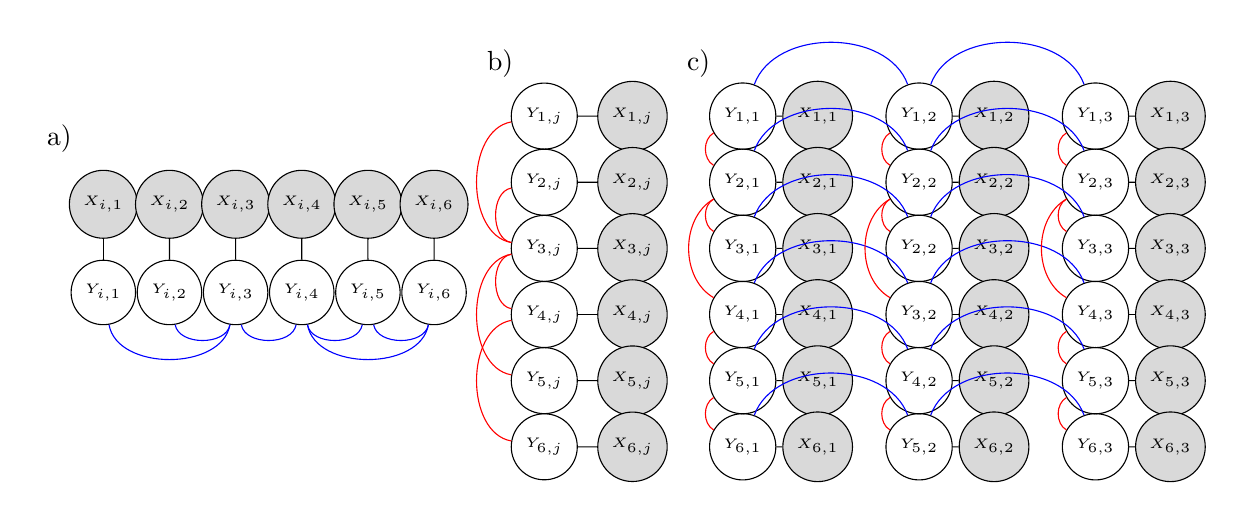
\begin{tikzpicture}[scale=0.56]
\tikzstyle{every node} = [draw, shape=circle]
\node[draw=none] (a) at (-1, 3.5) {a)};
\node (a) at (0, 0) {\tiny $Y_{i, 1}$};
\node (b) at (1.5, 0) {\tiny $Y_{i, 2}$};
\node (c) at (3, 0) {\tiny $Y_{i, 3}$};
\node (d) at (4.5, 0) {\tiny $Y_{i, 4}$};
\node (e) at (6, 0) {\tiny $Y_{i, 5}$};
\node (f) at (7.5, 0) {\tiny $Y_{i, 6}$};
\draw [-, draw=blue] (a) to  [out=280,in=260] (c);
\draw [-, draw=blue] (b) to  [out=280,in=260] (c);
\draw [-, draw=blue] (e) to  [out=280,in=260] (f);
\draw [-, draw=blue] (c) to  [out=280,in=260] (d);
\draw [-, draw=blue] (d) to  [out=280,in=260] (e);
\draw [-, draw=blue] (d) to  [out=280,in=260] (f);

\node [fill=gray!30](ax) at (0, 2) {\tiny $X_{i, 1}$};
\node [fill=gray!30](bx) at (1.5, 2) {\tiny $X_{i, 2}$};
\node [fill=gray!30](cx) at (3, 2) {\tiny $X_{i, 3}$};
\node [fill=gray!30](dx) at (4.5, 2) {\tiny $X_{i, 4}$};
\node [fill=gray!30](ex) at (6, 2) {\tiny $X_{i, 5}$};
\node [fill=gray!30](fx) at (7.5, 2) {\tiny $X_{i, 6}$};

\draw [-] (a) to  [out=90,in=270] (ax);
\draw [-] (b) to  [out=90,in=270] (bx);
\draw [-] (c) to  [out=90,in=270] (cx);
\draw [-] (d) to  [out=90,in=270] (dx);
\draw [-] (e) to  [out=90,in=270] (ex);
\draw [-] (f) to  [out=90,in=270] (fx);

\node[draw=none] (a) at (9, 5.2) {b)};
\node (a) at (10, 4) {\tiny $Y_{1,j}$};
\node (b) at (10, 2.5) {\tiny $Y_{2,j}$};
\node (c) at (10, 1) {\tiny $Y_{3,j}$};
\node (d) at (10, -0.5) {\tiny $Y_{4,j}$};
\node (e) at (10, -2) {\tiny $Y_{5,j}$};
\node (f) at (10, -3.5) {\tiny $Y_{6,j}$};

\node [fill=gray!30](ax) at (12, 4) {\tiny $X_{1,j}$};
\node [fill=gray!30](bx) at (12, 2.5) {\tiny $X_{2,j}$};
\node [fill=gray!30](cx) at (12, 1) {\tiny $X_{3,j}$};
\node [fill=gray!30](dx) at (12, -0.5) {\tiny $X_{4,j}$};
\node [fill=gray!30](ex) at (12, -2) {\tiny $X_{5,j}$};
\node [fill=gray!30](fx) at (12, -3.5) {\tiny $X_{6,j}$};

\draw [-] (a) to  [out=0,in=180] (ax);
\draw [-] (b) to  [out=0,in=180] (bx);
\draw [-] (c) to  [out=0,in=180] (cx);
\draw [-] (d) to  [out=0,in=180] (dx);
\draw [-] (e) to  [out=0,in=180] (ex);
\draw [-] (f) to  [out=0,in=180] (fx);

\draw [-, draw=red] (a) to  [out=190,in=170] (c);
\draw [-, draw=red] (c) to  [out=190,in=170] (d);
\draw [-, draw=red] (d) to  [out=190,in=170] (f);
\draw [-, draw=red] (b) to  [out=190,in=170] (c);
\draw [-, draw=red] (c) to  [out=190,in=170] (e);

\node[draw=none] (a) at (13.5, 5.2) {c)};
\node (a) at (14.5, 4) {\tiny $Y_{1,1}$};
\node (b) at (14.5, 2.5) {\tiny $Y_{2, 1}$};
\node (c) at (14.5, 1) {\tiny $Y_{3,1}$};
\node (d) at (14.5, -0.5) {\tiny $Y_{4, 1}$};
\node (e) at (14.5, -2) {\tiny $Y_{5, 1}$};
\node (f) at (14.5, -3.5) {\tiny $Y_{6, 1}$};

\node [fill=gray!30](ax) at (16.2, 4) {\tiny $X_{1, 1}$};
\node [fill=gray!30](bx) at (16.2, 2.5) {\tiny $X_{2, 1}$};
\node [fill=gray!30](cx) at (16.2, 1) {\tiny $X_{3, 1}$};
\node [fill=gray!30](dx) at (16.2, -0.5) {\tiny $X_{4, 1}$};
\node [fill=gray!30](ex) at (16.2, -2) {\tiny $X_{5, 1}$};
\node [fill=gray!30](fx) at (16.2, -3.5) {\tiny $X_{6, 1}$};


\draw [-] (a) to  [out=0,in=180] (ax);
\draw [-] (b) to  [out=0,in=180] (bx);
\draw [-] (c) to  [out=0,in=180] (cx);
\draw [-] (d) to  [out=0,in=180] (dx);
\draw [-] (e) to  [out=0,in=180] (ex);
\draw [-] (f) to  [out=0,in=180] (fx);

\node (a_) at (18.5, 4) {\tiny $Y_{1,2}$};
\node (b_) at (18.5, 2.5) {\tiny $Y_{2,2}$};
\node (c_) at (18.5, 1) {\tiny $Y_{2,2}$};
\node (d_) at (18.5, -0.5) {\tiny $Y_{3,2}$};
\node (e_) at (18.5, -2) {\tiny $Y_{4,2}$};
\node (f_) at (18.5, -3.5) {\tiny $Y_{5,2}$};

\node[fill=gray!30] (ax_) at (20.2, 4) {\tiny $X_{1,2}$};
\node[fill=gray!30] (bx_) at (20.2, 2.5) {\tiny $X_{2,2}$};
\node[fill=gray!30] (cx_) at (20.2, 1) {\tiny $X_{3,2}$};
\node[fill=gray!30] (dx_) at (20.2, -0.5) {\tiny $X_{4,2}$};
\node[fill=gray!30] (ex_) at (20.2, -2) {\tiny $X_{5,2}$};
\node[fill=gray!30] (fx_) at (20.2, -3.5) {\tiny $X_{6,2}$};

\draw [-] (a_) to  [out=0,in=180] (ax_);
\draw [-] (b_) to  [out=0,in=180] (bx_);
\draw [-] (c_) to  [out=0,in=180] (cx_);
\draw [-] (d_) to  [out=0,in=180] (dx_);
\draw [-] (e_) to  [out=0,in=180] (ex_);
\draw [-] (f_) to  [out=0,in=180] (fx_);

\node (a__) at (22.5, 4) {\tiny $Y_{1,3}$};
\node (b__) at (22.5, 2.5) {\tiny $Y_{2,3}$};
\node (c__) at (22.5, 1) {\tiny $Y_{3,3}$};
\node (d__) at (22.5, -0.5) {\tiny $Y_{4,3}$};
\node (e__) at (22.5, -2) {\tiny $Y_{5,3}$};
\node (f__) at (22.5, -3.5) {\tiny $Y_{6,3}$};

\node[fill=gray!30] (ax__) at (24.2, 4) {\tiny $X_{1, 3}$};
\node[fill=gray!30] (bx__) at (24.2, 2.5) {\tiny $X_{2, 3}$};
\node[fill=gray!30] (cx__) at (24.2, 1) {\tiny $X_{3, 3}$};
\node[fill=gray!30] (dx__) at (24.2, -0.5) {\tiny $X_{4, 3}$};
\node[fill=gray!30] (ex__) at (24.2, -2) {\tiny $X_{5, 3}$};
\node[fill=gray!30] (fx__) at (24.2, -3.5) {\tiny $X_{6,3}$};

\draw [-] (a__) to  [out=0,in=180] (ax__);
\draw [-] (b__) to  [out=0,in=180] (bx__);
\draw [-] (c__) to  [out=0,in=180] (cx__);
\draw [-] (d__) to  [out=0,in=180] (dx__);
\draw [-] (e__) to  [out=0,in=180] (ex__);
\draw [-] (f__) to  [out=0,in=180] (fx__);

\draw [-, draw=blue] (a) to  [out=70,in=110] (a_);
\draw [-, draw=blue] (a_) to  [out=70,in=110] (a__);
\draw [-, draw=blue] (b) to  [out=70,in=110] (b_);
\draw [-, draw=blue] (b_) to  [out=70,in=110] (b__);
\draw [-, draw=blue] (c) to  [out=70,in=110] (c_);
\draw [-, draw=blue] (c_) to  [out=70,in=110] (c__);
\draw [-, draw=blue] (d) to  [out=70,in=110] (d_);
\draw [-, draw=blue] (d_) to  [out=70,in=110] (d__);
\draw [-, draw=blue] (e) to  [out=70,in=110] (e_);
\draw [-, draw=blue] (e_) to  [out=70,in=110] (e__);
\draw [-, draw=blue] (f) to  [out=70,in=110] (f_);
\draw [-, draw=blue] (f_) to  [out=70,in=110] (f__);


\draw [-, draw=red] (a) to  [out=210,in=150] (b);
\draw [-, draw=red] (b) to  [out=210,in=150] (c);
\draw [-, draw=red] (b) to  [out=210,in=150] (d);
\draw [-, draw=red] (d) to  [out=210,in=150] (e);
\draw [-, draw=red] (e) to  [out=210,in=150] (f);

\draw [-, draw=red] (a_) to  [out=210,in=150] (b_);
\draw [-, draw=red] (b_) to  [out=210,in=150] (c_);
\draw [-, draw=red] (b_) to  [out=210,in=150] (d_);
\draw [-, draw=red] (d_) to  [out=210,in=150] (e_);
\draw [-, draw=red] (e_) to  [out=210,in=150] (f_);

\draw [-, draw=red] (a__) to  [out=210,in=150] (b__);
\draw [-, draw=red] (b__) to  [out=210,in=150] (c__);
\draw [-, draw=red] (b__) to  [out=210,in=150] (d__);
\draw [-, draw=red] (d__) to  [out=210,in=150] (e__);
\draw [-, draw=red] (e__) to  [out=210,in=150] (f__);
\end{tikzpicture}
\caption[Integrating similarity matrices]{\large{Integrating the similarity matrices: a) integration of only the target similarity matrix. The cells $Y_{i,1},\dots,Y_{i,6}$ indicate the predictions that are to be made for drug $d_i$. $X_{i,1},\dots, X_{i,6}$ indicate the predictions made by Matrix Factorization for those targets. Blue edges indicate similar targets. b) integration of only the drug similarity matrix. The cells $Y_{1,j},\dots,Y_{6,j}$ indicate the predictions that are to be made for target $t_j$. Red edges indicate similar drugs. c) integration of both similarity matrices. The cells $Y_{i,j}$ indicate the predictions that are to be made for the drug-target pairs in the cluster, consisting of drugs $d_1,d_2,d_3$ and targets $t_1,\dots,t_6$.}}
\label{fig:graph_structure}
\end{figure}


\subsection{Graphical structure of the CCRF}
As mentioned above, different strategies can be applied to chose the edges of the graphical model. Which of the \textit{CCRF} nodes are connected is defined through the similarity matrices $S^k$ in the formulation of the \textit{CCRF}. Theoretically, one can connect all nodes to all other nodes and weight the edges with the similarity between the corresponding drugs or targets. However, the time of computing the covariance matrix of the Gaussian distribution, which is defined through the \textit{CCRF} depends on the sparsity of the matrices $S^k$. It is necessary to compute this inverse in each step of the parameter learning as well as in the inference step. In order to get \textit{CCRFs} with a feasible structure, the edges for the experiments in this thesis where chosen by connecting all drugs and targets to its $k_{neighbors}=4$ nearest neighbors. 

%An other strategy to connect the nodes, that was tested in this thesis is to chose a similarity-threshold $t$ and connect all drugs and targets with a similarity above the threshold.

\subsubsection{Clustering of the Drug-Target Matrix}
Hierarchical clustering was utilized on the drug and target similarity matrices respectively to first cluster the drugs and targets into smaller subsets. For this task the R functions $hclust$ and $cutree$ were used. When clustering the drugs, based on the drug similarity matrix, $hclust$ initially assigns each drug to its own cluster and then proceeds iteratively, at each stage joining the two most similar clusters, until there is only one single cluster left, resulting in a tree as illustrated in figure \ref{davis_clustering}. The $cutree$ function with parameter $k_d$ then groups the clusters into $k_d$ disjunct sets of drugs. The same procedure is applied on the target similarity matrix resulting in $k_t$ disjunct sets of targets. Finally, we obtain $k_d \times k_t$ separate drug-target sets. For all $k_d$ drug sets we can now go over all $k_t$ target sets and construct a \textit{CCRF} for the submatrix of the respective drugs and targets. 

\begin{figure}[p]
\begin{center}
\includegraphics[scale=0.36]{davis_histogram.png}
\end{center}
\caption[Davis drugs clustering]{Clustering the drugs in the \textit{Davis} dataset, which is introduced in section \ref{sec:datasets}. The dendogram illustrates the similarities of the drugs in the \textit{Davis} dataset. The numbers at each leaf represent the drug indices. }
\label{davis_clustering}
\end{figure}


\section{Proof of Concept}

This section serves as a proof of concept for the model that is developed in this thesis. In a first step, a matrix of $n$ rows and $m$ columns is generated which is then partitioned into training and test data ($n$ simulated drugs and $m$ simulated targets). The matrix values are generated, such that the following assumptions are fulfilled:

\begin{itemize}
\item the dataset has underlying latent factors
\item there are certain pairs of columns in the generated dataset, s.th. the pairs of columns have similar values (simulating similar targets).
\end{itemize}

In a second step, a fraction of observations in this generated dataset is masked as test data. The remaining values are used as training data for the \textit{MF+CCRF} model. The model parameters are trained based on the training data and in the next step the values that were previously masked as test data are predicted. Finally, the performance of this model is evaluated in terms of Root Mean Square Error ($RMSE$) and compared to the performance of using only \textit{MF} or only \textit{CCRF}.
In the following, each of these steps is documented, starting with the simulation of the data.

\subsection{Data Simulation}
%\includegraphics[scale=0.3]{num_lf_mat.png}

A dataset of dimension $m \times n$ ($m$ drugs and $n$ targets) that has underlying latent factors and column-pairs with similar values can be simulated by first constructing a \textit{CCRF} and then taking a sample from it. At first, a matrix $X$ of size $m \times n$ is generated which has only underlying latent factors as shown in figure \ref{fig:numX}. Next, the graphical structure of the \textit{CCRF} is defined by arbitrarily choosing pairs of columns for which the \textit{CCRF} distribution should produce similar values. In the \textit{CCRF} formulation each matrix cell is a node and each node can be adjacent to any other node in the graphical model. Therefore the graphical structure of the \textit{CCRF} is defined by an adjacency matrix $B$ of size $mn \times mn$. Figure \ref{fig:numStructure} shows an example of a choice of structure for the \textit{CCRF}.  The values in matrix $X$ are used as node input for the \textit{CCRF}. Next $\alpha$ (importance of the node values) and $\beta$ (importance of the adjacency matrix) are chosen arbitrarily and a sample from the multivariate Gaussian distribution that can be derived from the \textit{CCRF} formulation as described in section \ref{sec:CCRF} is taken. This sample is used as the dataset for the numerical experiments. It has both underlying latent factors (because the input node values of matrix $X$ has underlying latent factors) and the assumption that \textit{similar targets} (which were chosen arbitrarily by defining the matrix $B$) have similar values is fulfilled. Figure \ref{fig:numSample} shows an example of a sample, taken from the multivariate Gaussian that is defined by the \textit{CCRF} where the structure of the model was chosen as described in figure \ref{fig:numStructure}.

%\includegraphics[scale=0.2]{num_lf_crf_mat.png}
%\includegraphics[scale=0.2]{num_train.png}
%\includegraphics[scale=0.2]{num_pred_mf.png}
%\includegraphics[scale=0.2]{num_pred_mf_crf.png}
\begin{figure}
\begin{center}
\includegraphics[scale=0.6]{numeric_X.png}
\end{center}
\caption[Sampling CCRF input]{\large{Sampling matrix $X$ which is used for the node input of the \textit{CCRF} distribution. First two latent-factor-matrices $LF_d$ and $LF_t$ of dimension $n \times k$ and $m \times k$, where $n$ is the number of drugs, $m$ is the number of targets and $k$ is the number of latent factors (here $k=10$ is chosen arbitrarily) are sampled randomly. $X$ is defined as the product $X=LF_d LF_t^T$ and is used as the values for the node input of the \textit{CCRF}.}}
\label{fig:numX}
\end{figure}

\begin{figure}
\begin{center}
\includegraphics[scale=0.6]{numeric_structure.png}
\end{center}
\caption[Defining the structure of the CRF]{\large{Defining the structure of the CRF. Assume each matrix cell is a node of the \textit{CCRF}. For the numerical experiments, the matrix columns where divided into groups of 10 columns. Each cell in each group was connected to all other cells in the same group, which is illustrated by the archs.}}
\label{fig:numStructure}
\end{figure}


\begin{figure}
\begin{center}
\includegraphics[scale=0.5]{numeric_sample.png}
\end{center}
\caption[Example of CCRF sample]{\large{Example of a dataset that is sampled from the \textit{CCRF} when the structure is chosen, such as described in figure \ref{fig:numStructure}. As can be seen, this dataset has the property that the nodes which are interconnected by the structure of the graphical model have similar values. Additionally this matrix has underlying latent factors because the node input values where generated by multiplying randomly sampled latent factor matrices.}}
\label{fig:numSample}
\end{figure}

\subsection{Experiments on Simulated Data}

For the numerical experiments a dataset of $n=40$ rows and $m=40$ columns was generated. As described above, for the dataset generation, a first dataset $X$ was generated which has only underlying latent factors. Next the \textit{CCRF} parameters were chosen arbitrarily as $\alpha=1$ and $\beta=2$. The graphical structure of the \textit{CCRF} was chosen as illustrated in figure \ref{fig:numStructure}. Next, the corresponding multivariate Gaussian was obtained, by first calculating the covariance matrix $\Sigma$ and mean vector $\mu$ as described in section \ref{sec:CCRF}. A sample from this distribution was taken as the simulated dataset which is visualized in figure \ref{fig:test1}. Next, around 120 training values were sampled from the complete dataset. An example of a sampled training dataset is shown in figure \ref{fig:test2}. First, Matrix Factorization was applied to predict the missing values and the $RMSE$ of the prediction was computed. Next, the \textit{CCRF+MF} model was applied to predict the missing values and the $RMSE$ was computed again for this prediction. The predictions of the \textit{MF} and \textit{MF+CCRF} model are visualized in figures \ref{fig:test3} and \ref{fig:test4}. The prediction of the \textit{CCRF} model without \textit{MF} as an initial prediction was also tested. As it is necessary to have \textit{some} node input $X$, the mean value of the training observations was used instead of the \textit{MF} prediction for the \textit{CCRF} model by itself. Table \ref{tab:x} lists the $RMSE$ of the methods and shows that the \textit{MF+CCRF} model outperforms the \textit{MF} and \textit{CCRF} models when used singularly.

\vspace{2cm}
\begin{table}[!ht]
\centering
\begin{tabular}{ c | c | c | c }
   & \textit{MF} & \textit{CCRF} & \textit{MF+CCRF} \\
$RMSE$ & 11.493& 11.909& 7.514   
\end{tabular}
\captionof{table}{$RMSE$ of $MF$, $CCRF$ and $MF+CCRF$ on simulated dataset.}
\label{tab:x}
\end{table}

\begin{figure}
\centering
\begin{minipage}{.5\textwidth}
  \centering
  \includegraphics[width=1\linewidth]{num_exp_ccrf_pred.png}
  \captionof{figure}{Generated dataset.}
  \label{fig:test1}
\end{minipage}%
\begin{minipage}{.5\textwidth}
  \centering
  \includegraphics[width=1\linewidth]{num_exp_train_data.png}
  \captionof{figure}{Training dataset.}
  \label{fig:test2}
\end{minipage}
\end{figure}


\begin{figure}
\centering
\begin{minipage}{.5\textwidth}
  \centering
  \includegraphics[width=1\linewidth]{num_pred_mf.png}
  \captionof{figure}{$MF$ prediction}
  \label{fig:test3}
\end{minipage}%
\begin{minipage}{.5\textwidth}
  \centering
  \includegraphics[width=1\linewidth]{num_pred_mf_crf.png}
  \captionof{figure}{$MF+CCRF$ prediction}
  \label{fig:test4}
\end{minipage}
\end{figure}

\subsection{Summary}
As pointed out in \ref{mod:intuition}, the idea of the combined \textit{MF+CCRF} model is that the \textit{CCRF} can improve the initial \textit{MF} prediction of a drug-target pair by interpolating from given observations of a similar drug on the same target or by interpolating from a given observation of a similar target on the same drug. For the numerical experiments, the first type of interpolation proved to be useful. The interpolation among the columns through the $CCRF$ improved the performance of using only $MF$ significantly. The $MF$ method alone does not capture the high correlation of the values inside the target groups as well as the combined method, which can be seen in figure \ref{fig:test3} and figure \ref{fig:test4}. The combined method also improves the performance of using the $CCRF$ alone. The reason for this is simple: some rows of the training dataset will not contain any observations for a complete target group (in figure \ref{fig:test2} for example the first row does not contain any observations for the second group of targets $t_{11},\dots,t_{20}$). When using only the $CCRF$ without $MF$ as an initial prediction, the prediction in these groups will be the mean value of the training data. When using $MF$ as an initial prediction instead, the $MF$ will have captured some information for these groups because of the underlying latent factors, which can be learned from the remaining target groups.

